% Status überarbeitet
% Status Zweitkorrekt 
\section{Analyse der statischen Ist-Architektur}

\subsection{Reverse Engineering}
Da die Ist-Architektur des FreeDesign-Editors zuvor kaum dokumentiert war, musste die aktuelle Architektur zunächst rekonstruiert werden. 
Dies wird als \emph{Reverse Engineering} bezeichnet und hat, laut der Definition von Chikofsky und Cross (\citeyear[S. 13-17]{Chikofsky1990}), zwei Ziele: 
\begin{itemize}
    \item Die Darstellung des Softwaresystem in einer abstrakten Form. 
    \item Die Identifikation der Komponenten eines Softwaresystems und ihre Beziehungen untereinander. 
\end{itemize}
Das Reverse-Engineering der Ist-Architektur de FreeDesign-Editor bezieht sich auf den Projektzustand vom 11. Januar 2020. 

\subsection{Darstellung des Softwaresystems}
Das Ziel war eine Form der Darstellung des Softwaresystems zu finden, die das Identifikation der Komponenten und ihrer statischen Zusammenhänge unterstützt.

\subsubsection{Das {dependency-cruiser}-Werkzeug}
Das Reverse Engineering kann durch den Einsatz von Analyse-Werkzeugen unterstützt werden, wobei üblicherweise ein einzelnes Werkzeug nicht alle Analyse-Aufgaben übernehmen kann \autocite[vgl.][381]{Bass2013}.  

Für die Visualisierung der Ist-Architektur wurde das Werkzeug \emph{dependency-cruiser}, welches von Sander Verweij entwickelt und unter \url{https://github.com/sverweij/dependency-cruiser} veröffentlicht wurde, in der Version v9.22.0 eingesetzt. 
Das Werkzeug untersucht das Verzeichnis, in dem der Quelltext eines TypeScript-Projektes enthalten ist und visualisiert die Struktur des Quelltextes als Abhängigkeitsgraph. Weiterhin können Regeln für die Abhängigkeiten der Komponenten angelegt werden, die durch das Werkzeug validiert, Verstöße gekennzeichnet und als Report ausgeben werden können \autocite[vgl.][]{Verweij:Dependency}. 

Das \emph{dependency-cruiser}-Werkzeug ist ein Programm für die Kommandozeile, welches mit unterschiedlichen Argumenten aufgerufen werden kann \autocite[vgl.][]{Verweij:CLI}.

\subsubsection{Konfiguration des dependency-cruiser-Werkzeug}
Für alle Analysen mit dem dependency-cruiser-Werkzeug wurde dieselbe Konfigurationsdatei angelegt, welche im Anhang unter \emph{W1\_dependency-cruiser-konfiguration.json} enthalten ist. Diese wurde beim Aufruf des Programms durch die Angabe des Argumentes \lstinline|--config| eingebunden.
\begin{lstlisting}[language={sh}, label=depcruise-config, caption=Aufruf des \emph{dependency-cruiser} mit eingebundener Konfigurationsdatei]
    npx depcruise --config W1_dependency-cruiser-konfiguration.json src
\end{lstlisting}
Die Konfigurationsdatei liegt im JSON-Format vor. 

Das JSON-Format ist ein sprachunabhängiges Format zum Austausch von Informationen, welches auf strukturierten Text basiert. Der Text ist ein serialisiertes Objekt oder Array, deren Werte vom Datentyp Objekt, Array, Nummer oder eine Zeichenkette sein können. Weiterhin sind die Literale \lstinline|null|, \lstinline|true| und \lstinline|false| valide Wertzuweisungen \autocite[vgl.][]{JSON:Einführung}.  

Die Konfigurationsdatei besteht aus einem JSON-Objekt mit der, in Listing \ref{list:dc-config} abgebildeten, Struktur.
\begin{lstlisting}[language=sh, label=list:dc-config, caption=Struktur der Konfiguration für das dependency-cruiser-Werkzeug]
{
    "options": {
        "tsConfig": Object,
        "webpackConfig": Object,
        "reporterOptions": Object,
        "exclude": { "path": Array }
    },
    "allowed": Array,
    "forbidden": Array
}
\end{lstlisting}

% options
Die Eigenschaften \lstinline|tsConfig| und \lstinline|webpackConfig| des \lstinline|options|-Objekts enthalten Informationen über die Konfiguration des TypeScript-Projekts. Über die Eigenschaft reporterOptions konnte Einfluss auf das Aussehen der Abhängigkeitsgraphen genommen werden. Für die Eigenschaft \lstinline|exclude| wurde ein Array mit Pfadangaben, die von der Analyse ausgeschlossen werden sollten, angelegt. Dies betraf Abhängigkeiten zu externen Javascript-Bibleotheken, die für die interne Architektur keine Rolle spielen sowie Daten für Unit-Tests und CSS-Dateien. 

% forbidden & allowed
Die Eigenschaften \lstinline|forbidden| und \lstinline|allowed| enthalten die Regeln zur Validierung der Abhängigkeiten zwischen den Quelltextkomponenten. 
Beide Arrays enthalten eine Liste von Objekten, deren Grundstruktur durch Listing \ref{list:dc-relation} dargestellt wird.

\begin{lstlisting}[language=sh, label=list:dc-relation, caption=Struktur der Objekte für die Arrays \lstinline|forbidden| und \lstinline|allowed|]
{
    "from": { "path": String | Array }
    "to": { "path": String | Array }
}
\end{lstlisting}
Der Eigenschaft \lstinline|path| kann entweder ein einzelner regulärer Ausdruck oder ein Array aus regulären Ausdrücken zugewiesen werden. 
Auf Basis der Ausdrücke untersucht das Werkzeug \lstinline|import|-Anweisungen innerhalb von TypeScript-Dateien. Dabei bezieht sich die Eigenschaft \lstinline|path| in \lstinline|from| auf importierende Dateien und die Eigenschaft \lstinline|path| in \lstinline|to| auf importierte Dateien \autocite[vgl.][]{Verweij:Rules}.

Die genaue Funktionsweise wird in Listing \ref{list:depcruise-example} anhand eines Beispiels illustriert und anschließend erläutert.
\begin{lstlisting}[language={sh}, label=list:depcruise-example, caption=Beispiel einer Abhängigkeitesrelation]
{
    "from": { "path": "^src/services" },
    "to": { "path": [
        "^src/core",
        "^src/store",
        "^src/actions/types/ApiActionTypes.ts",
        "^src/actions/types/ProductApiActionTypes.ts",
        "^src/actions/types/GuiActionTypes.ts"
    ]}
},
\end{lstlisting}
Das Beispiel stammt aus dem \lstinline|allowed|-Array und erlaubt somit, dass Quelltext der innerhalb des Ordners \lstinline|src/services| liegt, auf Quelltext innerhalb der in \lstinline|to| angeben Pfade zugreifen darf. 
Somit ist beispielsweise die Importangabe \newline  
\glqq\lstinline|import ApiRoutes from '../../core/api/ApiRoutes';|\grqq \newline
innerhalb der Datei \lstinline|src/services/designService/CustomerDesignService.ts| valide.

Den Objekten können noch weitere Eigenschaften zugewiesen werden, für das \lstinline|forbidden|-Array wurden lediglich noch die Möglichkeiten der Namenszuweisung und der Zuweisung des Schweregrades eines Fehlers genutzt. Für den Schweregrad wurden die Grade \emph{Warnung} (\lstinline|warn|) und \emph{Fehler} (\lstinline|error|) genutzt.

Zunächst wurden Abhängigkeiten, für die innerhalb des Teams Konsens bestand, dass es sie grundlegend nicht geben darf, in das \lstinline|forbidden|-Array eingetragen. Während der Analyse der Ist-Architektur wurden die bestehenden Abhängigkeiten überprüft und alle Abhängigkeiten, die für valide befunden wurden, in das \lstinline|allowed|-Array aufgenommen. Da es für die Abhängigkeiten nur lose, mündlich kommunizierte Regeln gab, konnten nur wenige Einschränkungen der Abhängigkeiten tatsächlich getroffen werden.  

Das \lstinline|forbidden|-Array wurde außerdem durch die Einträge 
\lstinline|no-orphans| und \lstinline|no-circular| ergänzt.

Der Eintrag \lstinline|no-orphans| dient zum Aufdecken von ungenutzten Quelltextbestandteilen, was für die Entwicklung der Soll-Architektur wichtig war.

Mit Hilfe der Option \lstinline|no-circular| konnten zyklische Abhängigkeiten aufgedeckt werden.

Anlehnend an Lilienthal (\citeyear[vgl.][88 - 90]{Lilienthal2019}) greifen bei zyklischen Abhängigkeiten Komponenten gegenseitig aufeinander zu und bedingen sich somit gegenseitig. 

\begin{figure}[H]
    \centering
    \caption{Beispiele für Abhängigkeiten basierend auf Lilienthal}
    \label{fig:exampleCircular}
    \begin{subfigure}[b]{.3\textwidth}
        \centering
        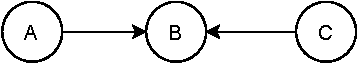
\includegraphics[width=.9\textwidth]{diagrams/Methoden/Circular-Example-C.pdf}
        \caption{ohne Zyklus}
        \label{fig:circularA}
    \end{subfigure}
    %\qquad
    \begin{subfigure}[b]{.3\textwidth}
        \centering
        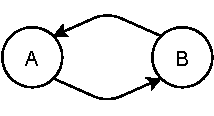
\includegraphics[width=.6\textwidth]{diagrams/Methoden/Circular-Example-A.pdf}
        \caption{mit Zyklus}
        \label{fig:circularB}
    \end{subfigure}
    %\qquad
    \begin{subfigure}[b]{.3\textwidth}
        \centering
        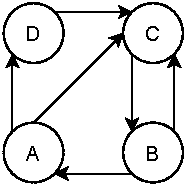
\includegraphics[width=.5\textwidth]{diagrams/Methoden/Circular-Example-B.pdf}
        \caption{Zyklusgruppe}
        \label{fig:circularC}
    \end{subfigure}
\end{figure}
In Abbildung \ref{fig:circularA} sind zwei zyklusfreie Abhängigkeiten illustriert, wobei A und B auf C zugreifen. Somit sind A und B von C entkoppelt. Eine Änderung an C hat Einfluss auf A und B, jedoch hat eine Änderung in A oder B keinen Einfluss auf C. Dadurch sind Abhängigkeiten leicht verständlich und problemlos erweiterbar. 
Auch lässt sich B isoliert von A und C testen. Für Tests von A und C kann B einfach simuliert werden.

Treten hingegen Zyklen in den Abhängigkeiten, wie in Abbildung \ref{fig:circularB} und \ref{fig:circularC} illustriert, auf, verringert sich die Verständlichkeit des Quelltextes und er lässt sich nur schwer ändern. Weiterhin lassen sich Komponenten in Zyklen schwer mit Unit-Tests testen und sind fehleranfällig \autocite[vgl.][116-117]{Martin2018}.

Bezogen auf Abbildung \ref{fig:circularB}, kann ein Änderung in A eine Änderung B zu Folge haben. Die Änderung in B kann wiederum eine Änderung in A notwendig machen. Somit können Änderung eine unerwünschte rückkoppelnde Wirkung haben.

Die durch das dependency-cruiser-Werkzeug aufgedeckten Zyklen zeigten Potenzial zur Verbesserung der Ist-Architektur auf und mussten bei der Entwicklung der Strategie zur Migration von Ist- in Soll-Architektur beachtet werden.

\subsubsection{Erzeugung eines Validierungsreports}
Mit dem in Listing \ref{depcruise-report} angeben Kommando wurde, auf Basis der in der Konfigurationsdatei hinterlegten Regeln, ein Validierungsreport erstellt.
Der Report enthält eine Liste aller Verstöße gegen die angegebenen Regeln.
\begin{lstlisting}[language={sh}, label=depcruise-report, caption=Kommando zur Erzeugung eines Validierungsreports]
npx depcruise --config W1_dependency-cruiser-konfiguration.json -T err-html src -f Validierungsreport.html
\end{lstlisting}

\subsubsection{Erzeugung der Visualisierungen}
Durch das Nutzen verschiedener Argumente konnten unterschiedliche Darstellungen der Ist-Architektur mit unterschiedlichem Fokus erzeugt werden. 

Zunächst wurde die Beziehung der Quelltextkomponenten auf der obersten Ordnerebene visualisiert und analysiert. 
Hierzu wurde das Werkzeug mit dem, in Listing \ref{list:depcruise-overview} angegebenen Kommando aufgerufen.

\begin{lstlisting}[language={sh}, label=list:depcruise-overview, caption=Kommando zur Erzeugung der Visualisierung der obersten Ordnerebene]
npx depcruise --config W1_dependency-cruiser-konfiguration.json -T archi src | dot -T svg > Projektuebersicht.svg
\end{lstlisting}

Für das Argument \lstinline|--output-type|, welches den Typen der Ausgabe angibt, wurde die Kurzform  \lstinline|-T| genutzt. Mit Hilfe des Typen \lstinline|archi| kann eine zusammenfassende Übersicht der Abhängigkeiten von Quelltext erstellt werden \autocite[vgl.][]{Verweij:Options}.

Die Visualisierung sämtlicher Abhängigkeiten der Software ergibt einen sehr umfangreichen und unübersichtlichen Graphen. Daher wurden mehrere Graphen erzeugt, die sich auf die Hauptaufgaben der Software beziehen:
\paragraph{Die Produktpräsentation} gehört zu den wichtigsten Aufgaben des FreeDesign-Editors. 
Sie ist als React-Komponente umgesetzt und der dafür verantwortliche Quelltext ist im Ordner 
\lstinline|src/components/pagePresenter| enthalten. Mit dem unter Listing \ref{depcruise-page-presenter} angegebenen Kommando konnten die Abhängigkeiten der Produktpräsentation visualisiert werden. 
\begin{lstlisting}[language={sh}, label=depcruise-page-presenter, caption=Erzeugung der Visualisierung der Abhängigkeiten für die Produktpräsentation]
npx depcruise --config W1_dependency-cruiser-konfiguration.json -T dot
  src/components/pagePresenter | dot -T svg > Produktpraesentation.svg
\end{lstlisting}

\paragraph{Die Designpräsentation} gehört ebenfalls zu den zentralen Aufgaben des FreeDesign-Editors und ist, wie die Produktpräsentation, als React-Komponente implementiert. Die Designpräsentation ist entkoppelt von der Produktpräsentation und wird dieser lediglich als Kindelement übergeben, wodurch das Design innerhalb der Produktpräsentation dargestellt werden kann.
Der für die Designpräsentation verantwortliche Quelltext ist im Ordner \lstinline|src/components/pagePresenter| hinterlegt. Die Abhängigkeiten der Designpräsentation wurden durch das, in Listing \ref{list:depcruise-design-presenter} angegebene, Kommando visualisiert.
\begin{lstlisting}[language={sh}, label=list:depcruise-design-presenter, caption=Erzeugung der Visualisierung der Abhängigkeiten für die Designpräsentation]
npx depcruise --config W1_dependency-cruiser-konfiguration.json -T dot 
  src/components/designPresenter | dot -T svg > Designpraesentation.svg
\end{lstlisting}

\paragraph{Das Editieren von Designs} ist die Kernaufgabe des FreeDesign-Editors. 
An dieser Funktionalität sind sehr viele Quelltextkomponenten des Editors beteiligt, die ausgehend vom Redux-Container \lstinline|Stage.tsx| zusammenarbeiten. Die Datei \lstinline|Stage.tsx| ist im Ordner \lstinline|src/containers/stage| hinterlegt, deren Abhängigkeiten durch das folgende, in Listing \ref{list:depcruise-design-edit} angegebene, Kommando visualisiert wurden.
\begin{lstlisting}[language={sh}, label=list:depcruise-design-edit, caption=Visualisierung der Abhängigkeiten für den Quelletext zum Editieren des Designs]
npx depcruise --config W1_dependency-cruiser-konfiguration.json -T dot  
  src/containers/stage | dot -T svg > Designeditieren.svg      
\end{lstlisting}
Da der Graph der Abhängigkeiten sehr umfangreich ist, wurde eine weitere kompakte Darstellung erzeugt (Listing \ref{list:depcruise-design-edit-compact}). Hierzu wurde das Argument \lstinline|--collapse| angewandt, welches einen Graphen der beteiligten Ordner erzeugt \autocite[vgl.][]{Verweij:CLI}. 

Der so erzeugte Graph bot einen wesentlich verbesserten Überblick der Beziehungen zwischen den beteiligten Komponenten.

\begin{lstlisting}[language={sh}, label=list:depcruise-design-edit-compact, caption=Kommando für eine kompakte Visualisierung der Abhängigkeiten von \lstinline|Stage.tsx|]
npx depcruise --config W1_dependency-cruiser-konfiguration.json --collapse 
  ".*/" -T dot src/containers/stage | dot -T svg > 
  Designeditieren-kompakt.svg
\end{lstlisting}

\paragraph{Die grafische Oberfläche} des FreeDesign-Editors
enthält, neben dem Redux-Container \lstinline|Stage.tsx|, eine Reihe weitere Elemente. Eine Übersicht der Elemente und der Abhängigkeiten wurden mit dem, in Listing \ref{depcruise-gui} angeben, Kommando erzeugen. Da sich der FreeDesign-Editor aus Redux-Container-Elementen zusammensetzt, die auf React-Komponenten, den Redux-State und Redux-Actions zugreifen, konnte die Analyse basierend auf dem Ordner \lstinline|src/containers| erfolgen. Da auch diese Visualisierung zu umfangreich sein würde, wurde ebenfalls \lstinline|--collapse| genutzt. Es wurde auch der Redux-Container Stage mit dem Argument \lstinline|--do-not-follow| ausblendet, da dessen Abhängigkeit bereits mit der vorangegangenen Visualisierung dokumentiert wurde.

\begin{lstlisting}[language={sh}, label=depcruise-gui, caption=Visualisierung der Zusammenhänge der grafischen Elemente des Editors]
npx depcruise --config W1_dependency-cruiser-konfiguration.json 
  --do-not-follow "^src/containers/stage" --collapse ".*/" -T dot 
  src/containers | dot -T svg  > 
  Grafische-Oberflaeche.svg
\end{lstlisting}

\paragraph{Das Konvertieren von Adobe-Illustrator-Dateien} in die FreeDesign-Designstruktur, welches als Kommandozeilenprogramm für den in Abschnitt \ref{sect:Integrationsprozess_Designvorlagen} beschrieben Integrationsprozess bereitgestellt wird, ist ebenfalls ein Teil des FreeDesign-Projektes. 
Das Kommandozeilenprogramm wird durch die Datei \lstinline|src/draftImporterCli.ts| umgesetzt, deren Abhängigkeiten durch das, in Listing \ref{list:depcruise-draft-import} angegebene, Kommando visualisiert werden konnten.
\begin{lstlisting}[language={sh}, label=list:depcruise-draft-import, caption=Visualisierung der Abhängigkeiten des Programms zum Import der AI-Dateien]
npx depcruise --config W1_dependency-cruiser-konfiguration.json -T dot 
  src/draftImporterCli.ts | dot -T svg > AI-Import.svg
\end{lstlisting}

\paragraph{Das Konvertieren von der FreeDesign-Designstruktur in SVG-Dateien} als Voraussetzung für das Erstellen der Vorschaubilder ist ebenfalls ein Teil des, in Abschnitt \ref{sect:Integrationsprozess_Designvorlagen} beschrieben, Integrationsprozesses.  
Das Kommandozeilenprogramm für diesen Schritt wurde im Ordner \lstinline|src/designToSvgCLI| umgesetzt. Die Abhängigkeiten wurden mit dem, in Listing \ref{list:depcruise-design-to-svg} angegebene, Kommando visualisiert.
\begin{lstlisting}[language={sh}, label=list:depcruise-design-to-svg, caption=Visualisierung des Kommandozeilenprogramms designToSvgCLI]
npx depcruise --config W1_dependency-cruiser-konfiguration.json -T dot 
  src/designToSvgCLI | dot -T svg > SVG-Konvertierung.svg
\end{lstlisting}

% Das Werkzeug dependency-cruiser unter einer MIT-Linzenz zu Verfügung gestellt, welche eine kostenfreien Nutzung garantiert \autocite[vgl.][]{Verweij:License}. 


\subsection{Identifikation von Bausteinen}
Starke und Hruschka bezeichnen die Komponenten eines Softwaresystems als Bausteine, die miteinander in Beziehungen stehen \autocite[vgl.][24]{Starke2011}. Diese Bezeichnung wird auch in der vorliegenden Diplomarbeit angewendet, um einer Verwechselung zwischen Softwarebausteinen und React-Komponenten vorzubeugen.

Mit Hilfe der Abhängigkeitsgraphen wurden die Bausteine, aus denen der FreeDesign-Editor besteht, identifiziert. 

Um Fragmente des Quelltextes den Bausteinen zuzuordnen, wurde ein kleines Werkzeug entwickelt, welches das Quellenverzeichnis rekursiv durchsucht. Zum einen sucht es nach Dateien mit der Bezeichnung \glqq\lstinline|_component.md|\grqq{} und zum anderen, innerhalb der Quelltextdateien, nach der Textphrase \glqq\lstinline|// @component{BAUSTEINNAME}|\grqq{}. 
Mit Hilfe der \lstinline|_component.md|-Dateien, deren einziger Inhalt der Name eines Bausteins ist, kann der Inhalt eines bestimmten Verzeichnisses einem Baustein zugeordnet werden. Einzelne Quelltextdateien können mit der Textphrase \glqq\lstinline|// @component{BAUSTEINNAME}|\grqq{} Bausteinen zugeordnet werden. Die Textphrase kann auch mehrfach innerhalb einer Datei enthalten sein, wodurch es möglich ist, eine Datei mehreren Bausteinen zuzuordnen. 

Das Ergebnis der Analyse ist eine tabellarische Zuordnung von Bausteinen zu Quelltext-Fragmenten in Form einer HTML-Datei. 
Der Entwurf der Soll-Architektur konnte somit auf der Auflistung der Bausteine basieren. Die Zuordnung der Quelletext-Fragmente der aktuellen Implementation half dabei die Beziehungen zwischen den Bausteinen zu ordnen und eine Mirgrationsstrategie zu entwerfen.

Das Werkzeug ist im Anhang unter \emph{W2\_Komponentenzuordnung} enthalten.